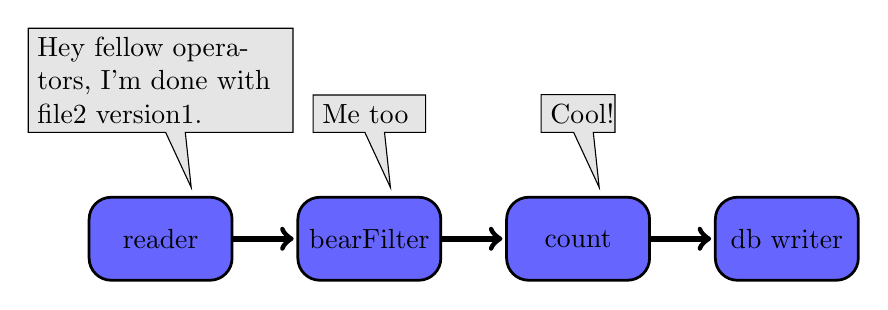
\begin{tikzpicture}[node distance = 0.8cm, auto]
\usetikzlibrary{shapes,arrows}
\usetikzlibrary{positioning}
\usetikzlibrary{calc,shapes.callouts,shapes.arrows}

\tikzstyle{operator} = [rectangle, draw, fill=blue!60, text width=4.5em, text centered, rounded corners = 8pt, minimum height=30pt, line width=1pt]
\tikzstyle{callout} = [draw, rectangle callout, callout relative pointer={#1}, line width=1pt]

    \node [operator] at (0, 0) (reader) {reader};
    \node [operator, right = of reader] (filter) {bearFilter};
    \node [operator, right = of filter] (count) {count}; 
    \node [operator, right = of count] (writer) {db writer};
    \node[draw, rectangle callout,callout relative pointer={(0.2cm,-0.7cm)},  text width=8.9em, aspect=2.5,fill=black!10, above = of reader] (hello) {Hey fellow operators, I'm done with file2 version1.};
    \node[draw, rectangle callout,callout relative pointer={(0.2cm,-0.7cm)},  text width=2em, aspect=2.5,fill=black!10, above = of count] (hello) {Cool!};
    \node[draw, rectangle callout,callout relative pointer={(0.2cm,-0.7cm)},  text width=3.4em, aspect=2.5,fill=black!10, above = of filter] (hello) {Me too};

    \draw [thick,->,shorten >=1pt, line width=2pt] (reader) -- (filter); 
    \draw [thick,->,shorten >=1pt, line width=2pt] (filter) -- (count);
     \draw [thick,->,shorten >=1pt, line width=2pt] (count) -- (writer); 


\end{tikzpicture}
